\documentclass{ctuthesis}
\usepackage{subfig}
\ctusetup{
	xdoctype = B,
	xfaculty = FCEyN,
	mainlanguage = czech,
	titlelanguage = czech,
	title-english = {Planting Uranium},
	title-czech = {Construcción e implementación de un sistema integral de 
	caracterización de filtros ópticos de interferencia de banda utilizados en 
	cámaras 
	hiperespectrales.},
	department-czech = {Departamento de Física},
	author = {Juan Reto Reynal},
	supervisor = {Prof. Dr. Hernán Grecco},
	supervisor-address = {Laboratorio de Electrónica Cuántica, DF, FCEyN, UBA.},
	month = 4,
	year = 2019,
}

\ctuprocess

\begin{abstract-english}
We develop \ldots
\end{abstract-english}

\begin{abstract-czech}
Rozvíjíme \ldots
\end{abstract-czech}

\begin{document}

\maketitle
\renewcommand{\chaptername}{Capítulo}
\renewcommand{\figurename}{Figura}
\chapter*{Plan de Tesis - Juan Reto Reynal}


\textsc{Título:} Construcción e implementación de un sistema integral de 
caracterización de filtros ópticos de interferencia de banda utilizados en 
cámaras 
hiperespectrales.


\hspace{-0.4cm}\textsc{Alumno:} Juan Reto Reynal L.U. 777/12.

\hspace{-0.4cm}\textsc{Director:} Dr. Hernán E. Grecco, Inv. Adj. CONICET, Prof. Adj. UBA.

\hspace{-0.4cm}\textsc{Lugar de trabajo:} LEC, Departamento de Física, FCEyN, UBA.


\section*{Objetivo general}
%conectar càmaras hiperespectrales con filtros y sus aplicaciones
%Como objetivo general se propone desarrollar métodos para optimizar la
%adquisición de imágenes hiperespectrales en las cuales se recopila y procesa, 
%con
%resolución espacial, información en un rango del espectro electromagnético. 
%Utilizando
%un modelo realista de adquisición que incluya parámetros tales como la 
%respuesta
%espectral del detector y la óptica así como también las características del 
%objeto
%observado, se optimizarán los métodos de sensado y deconvolución espectral. En
%particular se estudiará el efecto de variables físicas de relevancia, como por 
%ejemplo
%número de fotones, resolución espectral, resolución espacial y relación señal 
%ruido. En
%este trabajo, se estudiarán en particular la toma de imágenes hiperespectrales
%mediante sensores remotos y sus aplicaciones en la industria satelital.

%semrock:
\hspace{0.5cm} Los filtros ópticos utilizados en la construcción de cámaras 
hiperespectrales y 
multiespectrales resultan fundamentales en aplicaciones como la microscopía de 
fluorescencia \cite{Grecco2016} y la espectroscopía de reflectancia 
utilizada para la toma de 
imágenes hiperespectrales de la superficie de la Tierra \cite{Hogg2008}. En 
estas aplicaciones 
se distinguen claramente dos señales: una señal de entrada que viene dada por 
la iluminación (excitación) de una muestra ó la incidencia de la luz sobre la 
Tierra y, una señal de respuesta dada por la emisión en una muestra 
biológica ó la reflexión en el caso de la superficie de la Tierra.

Ambas señales no son solo espectralmente distintas sino que además difieren en 
su intensidad: la señal de entrada puede ser un millón de veces (o más aún) más 
intensa que la señal de respuesta (reflexión/emisión). En consecuencia, la 
capacidad de los filtros ópticos para transmitir ciertas longitudes de onda 
deseadas y bloquear el resto, resulta crítica para estas aplicaciones. Ahora 
bien, cuando el ancho de banda centrado en una cierta longitud de onda central 
que se desea transmitir es muy estrecho, las mediciones de las características 
espectrales y de transmisión de dichos filtros no suelen ser determinadas con 
precisión. Más aún, si los filtros son construidos especialmente por un 
proveedor (\textit{custom-made}) para una cierta aplicación específica, resulta 
fundamental su caracterización para decidir si incorporar o descartar dichos 
filtros a la carga útil de la aplicación en cuestión.

En el presente proyecto se propone desarrollar un sistema integral de 
caracterización de filtros de interferencia de banda con la capacidad de 
decidir si un filtro está apto o no para ser integrado a las cámaras 
hiperespectrales incorporadas en los satélites desarrollados por la empresa 
Satellogic.


%Optical filters play an important role in enabling applications such as 
%%%fluorescence
%microscopy and Raman spectroscopy. In these applications there are two 
%distinct types of
%beams: the illumination (or excitation) beam and the signal (or emission) 
%beam. 

%Not only are
%these beams spectrally distinct, but also they differ significantly in their 
%intensity – the signal
%beam can be a million times (or more) weaker than the illumination beam. 
%Therefore, the ability
%of filters to selectively transmit desired wavelengths of light while blocking 
%unwanted light is
%critical. The performance of such filters is determined by their spectral 
%characteristics, including
%transmission efficiency of the signal and attenuation (or blocking) of the 
%illumination light and
%undesirable emission wavelengths. In particular, often it is critical for 
%filters to transition from
%deep blocking to high transmission over a very short wavelength range, leading 
%to steep and
%deep spectral edges.
%However, due to limitations of standard metrology techniques, the
%measured spectral characteristics of thin-film interference filters are 
%frequently not determined
%accurately, especially when there are steep and deep edges.
%In this article we explore limitations to accurate filter spectrum 
%measurements with
%standard metrology techniques, and show how these limitations can be managed 
%by a better
%understanding of the limitations as well as more sophisticated measurements 
%when necessary.

\section*{Objetivos específicos del proyecto}
\begin{itemize}
	
	\item \texttt{Objetivo 0 - Abril:} Revisión del estado del arte.
	\item \texttt{Objetivo 1 - Mayo:} Armado de distintos setups de iluminación 
	o detección para distintas longitudes de onda para analizar los espectros 
	de transmisión de los filtros.
	\item \texttt{Objetivo 2 - Junio:} Armado de distintas configuraciones 
	experimentales controlando distintas formas de iluminar los filtros
	para poder encontrar los defectos.
	\item \texttt{Objetivo 3 - Agosto:} Construcción e implementación de un primer prototipo de un sistema integral que pueda decidir si un filtro está apto o no para ser integrado al satélite.
	\item \texttt{Objetivo 4 - Septiembre:} Establecer control de una de las cámaras de la empresa Satellogic para poder adquirir las
	imágenes. Procesar las imágenes tomadas haciendo HDR y búsqueda de características.
	\item \texttt{Objetivo 5 - Octubre:} Armado de un posible setup 
	experimental para poder caracterizar el filtro en su posición final
	en las cámaras de vuelo del satélite.
\end{itemize}
\section*{Antecedentes/Introducción **}
La captura de imágenes hiperespectrales consiste en colectar y procesar 
información en longitudes de onda específicas del campo electromagnético. El 
objetivo es obtener el espectro para cada pixel en la imagen de una escena, con 
el propósito de hallar objetos, identificar materiales y sustancias, o detectar 
procesos.
Los sensores hiperespectrales colectan información como un  set de imágenes. Cada una de ellas representa un rango estrecho de longitudes de onda del espectro electromagnético, el cual se conoce como banda espectral. Estas imágenes se combinan para formar un cubo de datos tridimensional (x,y,$\lambda$) para el procesamiento y análisis, donde x e y representan dos dimensiones espaciales de la escena, y $\lambda$ representa la dimensión espectral (la cual comprende a un cierto rango de longitudes de onda).
En los distintos sensores hiperespectrales, las longitudes de onda pueden ser separadas por diferentes tipos de filtros, o mediante el uso de instrumentos que sean sensibles a determinadas longitudes de onda, como por ejemplo interferómetros. La forma en la que las distintas longitudes de onda se combinan en un mismo pixel está intrínsecamente relacionada con el diseño particular del sensor que se emplee. Por este motivo, existe una estrecha relación entre el modelo de sensor que se emplee y el algoritmo de deconvolución requerido. Existen diversos diseños de sensores de escaneo multiespectral, algunos de los cuales se encuentran detallados a continuación [1]. Un resumen de estos diseños y sus respectivas SNR se puede encontrar en la referencia [3]. Otros métodos basados en técnicas de escaneo se pueden hallar en las referencias [4], [5] y  [6]. 

Espectrómetro de escaneo puntual (Point Scanning Spectrometer): El espectro incidente es dispersado a lo largo de un arreglo lineal de elementos de detección, permitiendo tasas de lectura muy rápidas. La escena es escaneada  a través del sensor mediante el empleo de dos espejos galvanométricos (o solamente uno en caso de que el sensor mismo se esté desplazando).

Espectrómetro de barrido (Pushbroom Spectrometer): el input del sensor es una abertura lineal, cuya imagen se dispersa a través de una matriz bidimensional de detectores, de forma que todos los puntos a lo largo de la línea son muestreados simultáneamente. Para completar la dimensión espacial ortogonal a la línea, la escena es escaneada a través de la apertura de entrada. Esto puede tener la forma de objetos moviéndose a través de una cinta transportadora, el suelo desplazándose bajo un satélite o una plataforma espacial, o la escena siendo escaneada a través de la rendija de entrada mediante un espejo galvanométrico.

Cámara de filtros tuneables (Tunable Filter Camera): una cámara de filtros tuneables se caracteriza por utilizar un sistema de filtros ajustables, ya sea eléctrica o mecánicamente. Entre estos sistemas se pueden destacar las ruedas de filtros, los dispositivos Fabry - Perot mecánicamente ajustables [7] [8], y los filtros ajustables tanto de cristal líquido (LCTF) [9] como los acusto ópticos (AOTF) [10], entre otros. Los tiempos de respuesta en el ajuste de los distintos filtros van desde $\approx$1 s para la rueda de filtros, $\approx$50 a 500 ms para el LCTF y el Fabry Perot mecánicamente ajustable, y $\approx$10 a 50 $\mu$s para el AOTF.

Espectrómetro de proyección de transformada de Fourier (Imaging Fourier Transform Spectrometer): se caracteriza por escanear un espejo de un interferómetro de Michelson con el objetivo de obtener mediciones para múltiples diferencias de camino óptico [11] [12]. Una alternativa más reciente es el espectrómetro de proyección de transformada de Fourier birrefringente, desarrollado por Harvey y Fletcher - Holmes, que cuenta con la ventaja de ser menos sensible a las vibraciones. [13]

Espectrómetro hiperespectral por tomografía computada (Computed Tomography Hyperspectral Imaging Spectrometer): es un dispositivo de escaneo similar a la técnica de snapshot CTIS, pero cuenta con la ventaja de ser capaz de colectar proyecciones provenientes de una mayor cantidad de ángulos, de forma que la data reconstruida tenga menos artefactos. La desventaja es que el detector no es usado eficientemente en comparación con otros métodos. [14]

Espectrómetro lineal de apertura codificada (Coded Aperture Line-Imaging Spectrometer): a pesar de que la espectrometría de apertura codificada comenzó como un método para escanear una apertura codificada a través de la rendija de entrada de un espectrómetro convencional, ha sido adaptada a arreglos bidimensionales modernos de detectores, dando lugar a una mejora en la relación señal - ruido. [15] [16]

El tamaño espacial de los pixels en sensores multiespectrales e hiperespectrales es en general lo suficientemente amplio como para que distintas sustancias puedan contribuir al espectro medido por un solo pixel. El objetivo de los algoritmos de deconvolución espectral consiste en extraer de un espectro los materiales constituyentes en la mezcla, así como las proporciones en las que aparecen. 
La deconvolución espectral es el procedimiento mediante el cual el espectro medido por un pixel es descompuesto en una colección de espectros constituyentes, endmembers, y un set de las correspondientes fracciones, abundancias, que indican la proporción de cada endmember presente en el pixel. Esto es importante en numerosos escenarios en los que el detalle a nivel subpixel es apreciable, los cuales pueden ir desde el campo de la microscopía de fluorescencia [17] (donde se detallan aplicaciones como Timelapse imaging [18] [19] y FRET [20], entre otras) hasta la toma de imágenes satelitales mediante sensores remotos. En el primer caso, los endmembers y las abundancias se pueden asociar a los fluoróforos y canales que se empleen, mientras que en las aplicaciones satelitales los endmembers normalmente corresponden a objetos macroscópicos en la escena, tales como agua, tierra, metal, o cualquier material natural o hecho por el hombre.
El proceso de deconvolución de principio a fin es en realidad una concatenación de tres procedimientos distintos, cada uno con objetivos específicos. La reducción dimensional reduce la cantidad de datos con el objetivo de disminuir la carga computacional en los pasos de procesamiento subsecuentes. La determinación de endmembers estima el set de distintos espectros que componen los píxeles mixtos en la escena. La etapa de inversión consta de proveer estimaciones de las abundancias fraccionales para los endmembers en cada pixel. 
La examinación del proceso de deconvolución se puede estudiar mediante tres criterios que categorizan estos algoritmos. 1. La interpretación de la data indica cómo un algoritmo interpreta el espectro combinado de un pixel. Principalmente se pueden distinguir dos clases de algoritmos, los estadísticos y los no estadísticos. 2. La descripción de la aleatoriedad indica cómo un algoritmo incorpora la aleatoriedad de los datos. Se pueden diferenciar según este criterio los métodos paramétricos de los no paramétricos. 3. Por último, el criterio de optimización indica cuál es la función objetiva que se está optimizando. Según este criterio, se pueden diferenciar los algoritmos que optimizan funciones tales como Squared error, Non squared error, Maximum a posteriori, Maximum likelihood, entre otras. [2]
\section*{Metodología}
Dentro del marco de esta investigación se realizarán las siguientes actividades. A través del estudio de papers y patentes acerca de los sistemas de sensado multiespectral existentes, se trabajará con los distintos algoritmos existentes de deconvolución espectral con el objetivo de familiarizarse con el estado del arte y conocer sus aplicaciones y restricciones. Se estudiará la aplicabilidad de cada uno de estos métodos en distintos casos. Para esto se cuenta con imágenes satelitales multiespectrales provistas por Satellogic. 
Paralelamente, se desarrollará un método de generación de imágenes satelitales multiespectrales artificiales que simule las características de la imagen relevantes para su adquisición. Las imágenes generadas se utilizarán para probar los algoritmos de deconvolución en cuestión. Finalmente se emplearán estos métodos en imágenes reales multiespectrales obtenidas de un microscopio confocal. 
El siguiente paso será el desarrollo de un algoritmo de deconvolución espectral óptimo que tenga en cuenta las variables físicas de relevancia en el sensado de imágenes, tales como el número de fotones, resolución espectral, resolución espacial y relación señal - ruido. En primer caso este estudio se hará para un caso genérico (lo cual tiene aplicaciones de suma importancia en microscopía, por ejemplo), y posteriormente se analizará el caso particular de sensores remotos, el cual presenta aplicaciones en la toma de imágenes satelitales. Las variables de interés serán determinadas en este caso mediante el análisis de imágenes satelitales existentes, las cuales serán provistas por Satellogic.
El software a desarrollar se encuentra intrínsecamente relacionado con el método de sensado que se emplee en la toma de las imágenes. El análisis del algoritmo desarrollado permitirá estudiar cuál es el método óptimo para la toma de imágenes multiespectrales, pudiendo aplicarse los resultados tanto a la microscopía como a la toma de imágenes satélitales por sensores remotos. El algoritmo de deconvolución se desarrollará en el lenguaje Python. 

\section*{Actividades asociadas al objetivo 1 - Mayo:}
\subsection*{ Armado de distintos setups de iluminación o detección para 
distintas longitudes de onda para analizar los espectros de transmisión de los 
filtros.}

\hspace{0.5cm}Debido a las limitaciones de las técnicas de medición estándard 
de los espectros de transmisión de los filtros ópticos donde se utilizan 
espectrómetros comerciales, las características de dichos 
filtros son determinadas generalmente de forma muy imprecisa, especialmente 
cuando el ancho de banda de transmisión centrado en una cierta de longitud de 
onda es muy estrecho (menos de una decena de nm para ciertas aplicaciones).


Como resultado de estas limitaciones, existen tres discrepancias fundamentales 
entre el espectro ''real''\footnote{El espectro ''real'' es 
el espectro de diseño del filtro para el que fue especialmente construido.} de 
un 
filtro y sus mediciones experimentales realizadas con 
espectrómetros comerciales (Ver Figura \ref{fig:obj1a})\cite{Semrock}. La 
primera discrepancia es el "redondeo" de características espectrales nítidas de 
los filtros. 
Esto se debe al ancho de banda no nulo del haz de la sonda del 
espectrómetro. La segunda discrepancia es el rango limitado de 
medición de la OD\footnote{La densidad óptica, OD (Optical Density), es un 
parámetro útil para describir la transmisión de la luz a través de un filtro 
óptico con una transmisión extremedamente baja. Si T es la transmisión del 
filtro, que varía entre 0 y 1, se define la densidad óptica como $OD = 
-$log$_{10} (T)$.} del filtro, que es 
	producto de la sensibilidad limitada del espectrómetro. 
	
	When a filter has high OD (such as OD > 6), very little light reaches the
	detector, and optical and electronic noise at the detector limit the lowest 
	signal that can be
	measured accurately. The signature of this artifact is a flat, noisy 
	spectrum that appears to be
	“pinned” to a certain OD value, despite the fact that the actual filter OD 
	can be substantially
	higher than the represented value. This signal limit is often called the 
	“noise floor,” and it can be
	wavelength dependent due to variations in the light source and detector 
	response spectra. Note
	that the noise floor can be decreased allowing for higher OD measurements 
	by opening up the
	monochromator slits and letting more light through the system, but this 
	increased sensitivity
	must be traded off against poorer spectral resolution.
	
	
	La tercera 
	discrepancia es propia de las mediciones de transiciones muy 
	pronunciadas. Esto surge 
	por el hecho de que el 
	haz de la sonda no es monocromático, sino que también tiene bandas 
	laterales débiles de longitudes de onda fuera de su ancho de banda 
	principal.

  
\begin{figure}[h!]
	\centering
	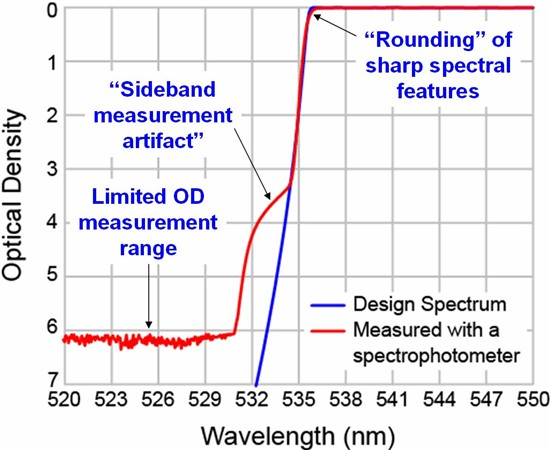
\includegraphics[scale=0.8]{Figs/plan_de_tesis/measurement_of_optical_filter.jpg}
	\caption{Discrepancias entre las mediciones experimentales con 
	espectrómetros 
	comerciales y el espectro ''real'' de un filtro óptico. Adaptado de 
	\cite{Semrock}.}
	\label{fig:obj1a}
\end{figure}

Ahora bien, dependiendo de la aplicación, las limitaciones en las mediciones 
del espectro de transmisión de los filtros pueden ser determinantes o no. En el 
presente proyecto se quiere determinar el arreglo experimental óptimo pero que 
sea compatible con los tiempos y costos de producción de la industria.

En ciertos filtros y aplicaciones, resulta de vital importancia el 
nivel de bloqueo de ciertos rangos de longitudes de onda pero no así la 
suavidad de la transición entre el bloqueo y la transmisión. Por ejemplo, en 
sistemas de 
imágenes de fluorescencia los espectros de absorción y emisión del fluróforo 
podrían estar lo suficientemente alejados como para que resulte fundamental que 
los filtros de banda de la señal de respuesta (de emisión) de la muestra tengan 
un bloqueo muy alto en la banda de la señal de excitación y así lograr una 
relación entre la señal y el ruido de adecuada proporción. 

Los filtros 
diseñados para estas aplicaciones podrían tener decenas de OD de bloqueo pero 
en 
la práctica incluso el más pequeño de los defectos físicos en los 
recubrimientos ópticos (\textit{coatings}) o en el montaje, así como el bajo 
nivel de control de luz parásita a nivel del sistema (**), puede limitar el 
bloqueo alcanzable a valores mucho menores que los del diseño original, en el 
rango de aproximadamente OD 6 a quizás 10.(forma indirecta de medir los scrath 
and dig!!**))) 

Dado que los espectrómetros 
comerciales estándard tienen una medición de OD de rango limitado debido al 
ruido de fondo del instrumento, se propone un arreglo experimental inicial para 
poder medir los niveles de bloqueo más altos con precisión como se muestra en 
la Figura \ref{fig:su} y que resulta compatible con la producción industrial 
deseada por su simplicidad.


\begin{figure}[h!]
	\centering
	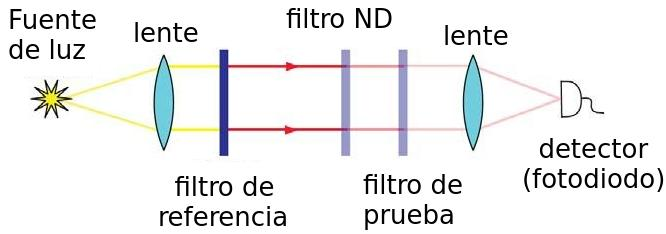
\includegraphics[scale=1.0]{Figs/plan_de_tesis/setup_u.jpeg}
	\caption{Arreglo experimental compatible con la producción industrial para 
	medir valores de 
	OD altos.}
	\label{fig:su}
\end{figure}

El método experimental de la Figura \ref{fig:su} se denomina 
\textit{complementary filter method}. Un haz de 
luz de banda ancha, de una lámpara QTH 
(\textit{Quartz-Tungsten Halogen}) ó de arco, aproximadamente colimado por una 
lente  es filtrado utilizando un filtro 
de referencia ampliamente bloqueador, que es esencialmente un filtro de banda 
con su banda de paso superpuesta a la región del espectro del filtro de prueba 
que se quiere analizar donde la medición de valores de OD altos son necesarios. 
La luz transmitida es enfocada con una lente convergente en un detector de bajo 
ruido capaz de medir niveles de intensidad de luz muy pequeños, como un 
fotodiodo de gran área con un circuito amplificador de bajo ruido ó un tubo 
fotomultiplicador (PMT).


Las mediciones se realizan de la siguiente manera. En primer lugar, se mide la 
intensidad de la señal en el detector con solo el filtro de referencia y un 
filtro calibrado de densidad neutra (ND) en la trayectoria de la luz. El filtro 
ND sirve para reducir el nivel de la intensidad de la luz en el detector en 
una cantidad calibrada de forma tal que el bias \footnote{El bias del 
detector es el valor medido por el instrumento cuando no hay ninguna fuente 
de luz incidiendo sobre él, es el valor de \textit{offset} que se le suma a 
cualquier 
medición.} del rango 
dinámico limitado alcanzable por el detector sea reducido para alcanzar los 
niveles de la señal que el detector va a ver cuando se coloquen los filtros de 
prueba. En particular, con un filtro ND 3, el rango dinámico del detector tiene 
que ser de $10^{6}$ para medir hasta un valor de OD 9 de bloqueo. En segundo 
lugar, se retira el filtro ND y se lo reemplaza por el filtro de prueba para 
realizar una nueva medición de la intensidad con el detector. El cociente entre 
las dos mediciones de intensidad de la luz es igual al valor de OD del filtro 
de prueba, en el rango espectral del filtro de referencia.


\section*{Actividades asociadas al objetivo 2 - Junio:}
\subsection*{Armado de distintos setups de iluminación 
	o detección para distintas longitudes de onda para analizar los espectros 
	de transmisión de los filtros.}

The actual blocking provided by a filter is determined not only by its designed 
spectrum, but
also by physical imperfections of the filter, such as pinholes generated during 
the thin-film
coating process, dirt and other surface defects, or flaws in the filter 
mounting. Pinholes can
allow light to pass through the filter unblocked – a single 10 $\mu$m pinhole 
(that 
penetrates
completely through the coating) limits the blocking of a 10 mm diameter beam to 
at most OD 6,
regardless of the designed level of blocking of the filter spectrum. Other 
surface and mounting
imperfections can cause scattered light that ''leaks'' through the filter due 
to 
a shift of the
spectrum to a region of high transmission for scattered light at high angles of 
incidence, or via unblocked paths near the edges or mounting. Therefore, it is 
important to evaluate the blocking
performance of filters after they have been fully manufactured into finished 
products.
%\section*{Actividades asociadas al objetivo 3 - Agosto:}
%\subsection*{Construcción e implementación de un primer prototipo de un 
%sistema 
%integral que pueda decidir si un filtro está apto o no para ser integrado al 
%satélite.}


%\section*{Actividades asociadas al objetivo 4 - Septiembre:}
%\subsection*{Establecer control de una de las cámaras de la empresa Satellogic 
%para poder adquirir las
%	imágenes. Procesar las imágenes tomadas haciendo HDR y búsqueda de 
%	características.}


%\section*{Actividades asociadas al objetivo 5 - Octubre:}
%\subsection*{Armado de un posible setup 
%	experimental para poder caracterizar el filtro en su posición final
%	en las cámaras de vuelo del satélite.}

\section*{Factibilidad}

\hspace{0.5cm}El lugar de trabajo donde el tesista va a desarrollar sus 
actividades es el 
Laboratorio de Electrónica Cuántica (LEC) del Departamento de Física de la 
Facultad de Ciencias Exactas y Naturales, UBA. El LEC cuenta con todas las 
instalaciones, infraestructura, instrumentos de medición y equipamiento 
necesarios para llevar a cabo la presente tesis. 

El director de la presente tesis es director del LEC y es experto en temas de 
óptica y fotofísica, áreas principales del proyecto. Además, tiene la 
experiencia de haber dirigido a una estudiante que realizó la tesis en conjunto 
con el LEC y la empresa Satellogic, resultando en una experiencia exitosa.

El tesista se encuentra cursando actualmente sus últimas dos materias de la 
carrera: 
Estructura de la Materia 4 e Instrumentación y Control.

El tesista junto a su director firmarán un NDA (Non-Disclosure Agreement) que 
le permitirán acceder a información importante para lograr el presente proyecto 
de tesis.**

\section*{Referencias}
1. [Hagen 2013] Nathan Hagen , Michael W. Kudenov. Review of snapshot spectral imaging technologies. Optical Engineering 52(9), 090901.

2. [Keshava 2003] Nirmal Keshava. A Survey of Spectral Unmixing Algorithms. Lincoln Laboratory Journal, Vol. 14, 1, 2003.

3. [Sellar 2005] R. G. Sellar and G. D. Boreman, “Comparison of relative signal-tonoise
ratios of different classes of imaging spectrometer,” Appl. Opt. 44(9), 1614–1624 (2005).

4. [Eismann 2012] M. T. Eismann, Hyperspectral Remote Sensing, SPIE Press, Bellingham, WA (2012).

5. [Harvey 2000] A. R. Harvey et al., “Technology options for imaging spectrometry,”
Proc. SPIE 4132, 13–24 (2000).

6. [Prieto 2008] X. Prieto-Blanco et al., “Optical configurations for imaging spectrometers,” Comput. Intell. Rem. Sens. 133, 1–25 (2008).

7. [Atherton 1981] P. D. Atherton et al., “Tunable Fabry-Perot filters,” Opt. Eng. 20(6),
806–814 (1981).

8. [Antila 2012] J. Antila et al., “Spectral imaging device based on a tuneable MEMS
Fabry-Perot interferometer,” Proc. SPIE 8374, 83740F (2012).

9. [Gupta 2008] N. Gupta, “Hyperspectral imager development at Army Research
Laboratory,” Proc. SPIE 6940, 69401P (2008).

10. [Poger 2001] S. Poger and E. Angelopoulou, “Multispectral sensors in computer
vision,” Technical Report CS 2001-3, Stevens Institute of Technology (2001).

11. [Potter 1972] A. E. Potter, “Multispectral imaging system,” U.S. Patent No. 3702735 (1972).

12. [Descour 1996] M. R. Descour, “The throughput advantage in imaging Fouriertransform spectrometers,” Proc. SPIE 2819, 285–290 (1996).

13. [Harvey 2004] A. R. Harvey and D. W. Fletcher-Holmes, “Birefringent Fourier-transform imaging spectrometer,” Opt. Express 12(22), 5368–5374 (2004).

14. [Mooney 1995] J. M. Mooney, “Angularly multiplexed spectral imager,” Proc. SPIE
2480, 65–77 (1995).

15. [Fernandez 2007] C. Fernandez et al., “Longwave infrared (LWIR) coded aperture
dispersive spectrometer,” Opt. Express 15(9), 5742–5753 (2007).

16. [Gehm 2008] M. E. Gehm et al., “High-throughput, multiplexed pushbroom hyperspectral microscopy,” Opt. Express 16(15), 11032–11043 (2008).

17. [Zimmermann 2005] Timo Zimmermann. Spectral Imaging and Linear Unmixing in Light Microscopy. Adv Biochem Engin/Biotechnol (2005) 95: 245– 265

18. Shima DT, Scales SJ, Kreis TE, Pepperkok R (1999) Curr Biol 9:821 

19. Ellenberg J, Lippincott-Schwartz J, Presley JF (1999) Trends Cell Biol 9:52

20. [Wouters 2001] Wouters FS, Verveer PJ, Bastiaens PI (2001) Trends Cell Biol 11:203
\chapter{Conclusion}

Lorep ipsum \cite{doe}


\renewcommand\bibname{Referencias Bibliográficas}
\begin{thebibliography}{1}

\bibitem{Grecco2016} Hernán E. Grecco, Sarah Imtiaz y Eli Zamir. Multiplexed
imaging of intracellular protein networks. 2016.

\bibitem{Hogg2008} David W. Hogg y Dustin Lang. “Astronomical imaging: The
	theory of everything”. AIP Conference Proceedings. Vol. 1082.
	2008, págs. 331-338. \href{https://arxiv.org/pdf/0810.3851.pdf}{arXiv: 
	0810.3851.}

\bibitem{Semrock} Turan Erdogan y Prashant Prabhat. Semrock Technical Note 
Series: Measurement of 
Optical Filter Spectra. 

\end{thebibliography}

\end{document}

